\documentclass[11pt, a4paper]{report}

\usepackage[utf8]{inputenc}
\usepackage{graphicx}%Required for graphics.
\usepackage{enumitem} %Used for modifing the labels used for items in lists. http://mirror.ox.ac.uk/sites/ctan.org/macros/latex/contrib/enumitem/enumitem.pdf
\usepackage{hyperref} %Used for hyperlinks to reference materials, and section referencing.
\usepackage{tabulary} %used for tables.
\usepackage{booktabs} %Used for nicer table formatting eg midrule

%This package gives us sideways figures and tables
\usepackage{rotating}

\usepackage{float}		%Gives the "H" placement command, which really means here - not here if it fits. Will start new page if required.
%E.G. \begin{figure}[H] will appear exactly there in the document, preceeded and succeeded by exactly what you'd expect

\usepackage[british]{babel} %biblatex treats english (the default) as American, and ruins the dates. Thus this is necessary to fix that.
\usepackage[backend=biber, citestyle=authortitle, style=authortitle]{biblatex}

\def\sectionautorefname{Section}
\def\subsectionautorefname{Subsection} % Reassigning the default names to have capitals.

%The command gives hyperlinked referencings in the form Section #: SectionTitle
\newcommand{\gref}[1]{\hyperref[#1]{\autoref*{#1}: \nameref{#1}}} % Good referencing = gref

\def\itempar#1\\{\item \textbf{#1}\\} %Macro to automatically bold the first line of an item in a list. Usage is \itempar Line1\\ Line 2...N

\addbibresource{sources.bib}

\begin{document}

\chapter{System Requirements Specification}

\tableofcontents
\pagebreak

\section{Introduction} \label{sec:Intro}

This document outlines the requirements, scope, and boundaries placed upon the project based on an interpretation of the document \href{http://www.macs.hw.ac.uk/~rpp6/teaching/GroupProject/docs/project/GroupProjectSpec2017.pdf}{"Year 3 Group Project Specification - Restaurant Ordering System"}

\section{Purpose} \label{sec:purpose}

The purpose of this system is to support restaurant staff in taking and fulfilling food orders from customers. The system is intended to make the process of relaying orders to the kitchen and fulfilling them more efficient, whilst increasing the information available to customers regarding their order. The aim is to allow servers to take quickly take complex orders from a customer or group of customers and have this automatically relayed to kitchen staff. The kitchen staff will then be able to provide certain feedback on the order, such as estimated time to delivery, which will be viewable by customers through this system.

\section{Scope} \label{sec:Scope}
The Restaurant Ordering Support System (henceforth "The system", or "ROSS"), will be designed to receive orders from waiting staff and relay this information to staff working in the kitchen. ROSS will also allow waiting staff to amend orders, kitchen staff to provide feedback on orders (for example, the time until delivery), and customers to view some or all of this feedback alongside their order details. This is to achieve the aim of increasing operational efficiency at the restaurant and customer experience.\\
\\
The system will also be designed to handle a good variety of data to support the client's need to deploy the system across multiple differing restaurant environments.\\
\\
The system will not be designed to provide detailed instructions on the preparation of food, only what dishes have been ordered (with any modifications). It will also not implement a stock management system, though some emulation of such a system may be implemented.\\
No aspect of the system will process payments from customers, though price information about items on the menu may be represented in the system. The system will also not be explicitly designed to integrate with any other technologies the restaurant may be using, for example, Point of Sale or Stock Control systems.

\section{Overview} \label{sec:Overview}
\subsection{Context} \label{subsec:Context}

The system will interact with 3 existing groups of people:
\begin{enumerate}
\item Waiting Staff\\
These are the people who converse with customers to elicit instructions for the kitchen staff to act upon. These instructions are usually in the form of food and/or drinks orders, or amendments to previously made orders. In the existing system, they are also responsible for relaying information from the kitchen staff to a customer. Waiting staff may or may not deliver food from the kitchen to customers.
\item Kitchen Staff\\
This group consists of any person responsible for the preparation of food or drink for customer consumption.
\item Customers\\
Anyone who enters the restaurant's premises with the intent to purchase food or drink is considered a customer. The System is only concerned with formalising a customer's request, not with encouraging or eliciting purchases.
\end{enumerate}

\noindent
These groups of people (collectively "users") will interface with ROSS through one of five distinct software components:
\begin{enumerate}
\item A Kitchen component to display information on current, unfulfilled orders to kitchen staff. The component will also be responsible for processing input to the system from the kitchen staff.
\item A Waiting component to allow waiting staff to enter, view, and amend customers' orders into the system.
\item A Customer component allowing customers to view the current status of their order. Any other direct interaction between the system and any customer (I.E. not through another user) will be the responsibility of this component.
\item A Database component responsible for storing any persistent information required by the system. For example all current unfulfilled orders, the restaurant's menu, and the availability of items on it. These examples will not necessarily be required by or implemented in the system.
\item A Server component which will manage the flow of information between the four previously mentioned components.
\end{enumerate}

\noindent
The general process of interaction expected is for a customer to converse with a member of Waiting staff to place or amend an order, or to request an update on their existing order. This member of Waiting staff will then interact with the system to formalise the customer's request through the Waiting component. The staff member will then receive some information from that same component regarding the request; for example, "Accepted", "Denied", details of an order, etc. These details can then be acted upon by the staff member or customer.\\
When a request has been formalised in this manner, the request is passed from the Waiting component to the Server component, which will act upon the request and interact with other components as required. Interaction with the Database component will usually be related to either recording the request for possible future use within or outwith the system, or to confirm such a request is valid or feasible.\\
\\
In the case of new orders being placed or existing orders amended, the relevant details from the request will be passed from the Server component to the Kitchen component.\\
This component, in relaying order details to the kitchen staff, allows them to prepare the food or drink as requested by the customer. It will also allow them to provide information related to the request to ROSS, which will then act accordingly.\\
\\
The customer's direct interaction with the system will include viewing the status of their order. That is the formalisation of their order recorded by ROSS, and some or all of the related information provided by the kitchen staff. Further interaction may or may not form part of the system as finally implemented.
\\
\\
Interaction with the aforementioned software components will take place through hardware owned and operated by the customer (for the Customer component) or provided by the restaurant in all other cases.\\
Interfaces between the components will utilise standard web technologies and practices as described in \gref{sec:Interfaces}.

\subsection{Functions} \label{subsec:Functions}

System functions are discussed generally in \gref{subsec:Context} and specifically in \gref{sec:Functional}

\subsection{User Characteristics} \label{subsec:Characteristics}
Expanding on the user groups defined in \gref{subsec:Context}, their use of the system can be further defined as follows:

\begin{enumerate}
\item \textbf{Waiting Staff} \\This group will interact with the system through a mobile wireless device, most likely in the form of a tablet computer. Each member of the group will have a device. Given the number of staff members varies by restaurant, the size of this group is unknown; however it is not expected for there to be any more than 20 such people at any given time. This group consists only of Waiting staff who are working at the time in question.\\
\\
It is expected that with their regular usage this group will become familiar with the system's interface design (the Waiting component particularly), its functionality and limitations. As such the Waiting component can rely more heavily on implicit knowledge, making it more efficient to use through a simpler interface.\\
There is a distinct possibility that certain aspects of the interface could be operated without looking at it given enough experience, and the design will aim to maximise this possibility.\\
Using the system both on a regular basis multiple times a day and in relation to employment, this group likely place ease of use and functionality significantly higher than visual aesthetics. They likely do not want to enjoy the interface per se, rather they want it to be second nature and make no investment - physical or mental - in its operation.


\item \textbf{Kitchen Staff}\\
The kitchen staff also will make regular usage of the system multiple times a day in their employment. However their requirements are subtly different. In the potentially hectic and high-pressure environment of a kitchen, the interface (Kitchen component) must require a minimal amount of time and thought to operate. The aesthetics must also be carefully considered in order to convey as much information as possible without requiring appreciable concentration - it should work well with only glances from the staff.\\
While implicit knowledge can be assumed through experience, 'blind' operation will likely not feature due to the changing nature of the information being displayed.\\ 
\\
This group will utilise a number of touch-screen devices of a size roughly according to an average desktop PC monitor. These will be installed in the kitchen itself in fixed locations, and may be shared amongst members. As such the size of kitchen is the determining factor rather than the number of staff. An amount from 1 to 5 would be considered normal, with anything up to 10 devices being reasonably expected.


\item \textbf{Customers}\\
Unlike other groups, the customers will not make regular usage of the system, and will not likely use it constantly throughout the day. As such they likely place a relatively high value on the aesthetics and enjoyment from using the system, and are willing to sacrifice some aspects of usability or functionality. That is not to say those aspects can be neglected.\\
As a consequence, customers will require much more prompting and signposting from the system to help formalise their intent. Given their intermittent usage, customers will willingly pay more attention to the interface and afford more deliberation in their actions. This reduces the requirement for a slick and intuitive interface relative to the Kitchen and Waiting staff members.
\end{enumerate}



%%%%%%%%%%%%% Start of Functional Requirements %%%%%%%%%%%%%




\section{Functional Requirements} \label{sec:Functional}

\begin{enumerate}[label=F-UR-\arabic*, series=functional]

\itempar \label{req:PlaceOrder}Allow waiting staff member to place customers' orders\\
Priority: Variable\\
Highest Priority: Must Have\\
Source: \href{http://www.macs.hw.ac.uk/~rpp6/teaching/GroupProject/docs/project/GroupProjectSpec2017.pdf}{"Group Project Specification Document"}

\begin{enumerate}[label*=.\arabic*]
\itempar \label{req:EnterID}Allow staff member to enter unique identification\\
\underline{\smash{Priority: Must Have}}\\
The system will accept from the staff member 1 or more pieces of information that will allow the order to be uniquely identified by both staff member and customer. These details will be some combination of:
\begin{itemize}
\item Any part of the customer's name. Forename, surname, nick-name, pen name and similar are all acceptable.
\item Group Number. A number determined by the restaurant to group relevant orders together. For example, using a table number allows multiple separate orders by different people to be logically grouped.
\item Unique Order Number. A number specific and unique to the order to which it is assigned. This is the only detail allowed to be used by itself.
\end{itemize}
The unique ID should be easily memorable by the customer. It is preferred if the customer has some reference to the Group Number or Unique Order Number eg. Number marked on the table.

\itempar \label{req:getMenu}Present staff member with restaurant menu\\
\underline{\smash{Priority: Must Have}}\\
Show to the staff member the menu of the restaurant in a hierarchical manner.\\
The position of elements displayed to the person should be consistent for any number of orders where the menu hierarchy has not been modified, and for any location in that hierarchy.

\itempar Allow staff member to navigate the menu and select an item\\
\underline{\smash{Priority: Must Have}}\\
The staff member must be able to navigate the menu hierarchy in an arbitrary order, able to revisit and/or return to a previous location in the hierarchy.\\
They must also be able to select any item from the menu, and to return to the menu from that selection. The location in the menu they return to should be the same location from which they made the selection.

\itempar \label{req:OrderRequests}Allow staff member to record arbitrary details regarding selected item\\
\underline{\smash{Priority: Must Have}}\\
After selecting an item, the person must be able to record any arbitrary requests made by the customer regarding the item. This may include, but is not limited to: 
\begin{itemize}
\item Requests to omit items (eg remove cheese from a burger)
\item Requests to add or substitute items (eg swap chips for curly fries)
\item Acknowledgement of dietary or allergy requirements (eg peanut allergy)
\item Selection from options listed on menu (eg cake with choice of custard or ice cream)
\end{itemize}
It must also be possible to record the amount of said item to be ordered. Where some arbitrary detail/request has been recorded, for example to omit cheese, that detail should be applied to \textbf{all} of the items specified by the amount recorded. So for example if the request "No cheese" and the amount "5" are recorded for an item "burger", the order should consist of 5 burgers of which \textbf{none} have cheese.

\itempar \label{req:ConfirmOrder}Forming and placing order for fulfilment\\
\underline{\smash{Priority: Must Have}}\\
The staff member must be able to select and record details for a number of different items and have the system remember all previous selections and their details. Additionally they must be able to view this list of selections (defined as an order), and remove items from it.\\
They must be able to place this order for fulfilment, such that information recorded by the system is displayed pursuant to \autoref{req:KitchenDisplay}.\\
The exact number of items an order may contain is specified in \autoref{per:OrderSize}.

\itempar \label{req:AutoGroup}Automatically grouping items in an order\\
\underline{\smash{Priority: Could Have}}\\
The system could automatically group certain menu items together in the order and show these groups as part of \autoref{req:KitchenDisplay}, with the aim of all the items in a group being complete and delivered to the customer at approximately the same time. For example, it could group starters, mains, and desserts into separate groups such that each group is individually prepared and served sequentially.

\itempar \label{req:ManualGroup}Specify item groupings in an order\\
\underline{\smash{Priority: Should Have}}\\
Similar to \autoref{req:AutoGroup} and in addition to \autoref{req:OrderRequests} above, the system should separately and explicitly record groupings of items within an order. Any specified grouping must override any automatic grouping that may otherwise be made by the system under \autoref{req:AutoGroup}.
\end{enumerate}


\itempar \label{req:AmendOrders}Allow waiting staff to amend existing orders\\
Priority: Must Have\\
Source: \href{http://www.macs.hw.ac.uk/~rpp6/teaching/GroupProject/docs/project/GroupProjectSpec2017.pdf}{"Group Project Specification Document"}
\begin{enumerate}[label*=.\arabic*]
\itempar \label{req:RetrieveOrder}Retrieve order details\\
The system must request the unique identification details entered as part of \autoref{req:EnterID} from the user.\\
If these details are invalid, the system must notify the user and prompt again for input.\\
There is no expectation for the system to check if the details refer to the intended order.\\
\\
Once a valid (but not necessarily 'correct') set of ID details has been received, the system must display the details of the order (to which the entered ID details refer) to the user. The system is not required to display all stored information regarding the order, only that which is considered pertinent.

\itempar Amend or Remove order details\\
With an order being displayed to the user, they must be able to select any item in the order and change any associated details recorded as part of \autoref{req:OrderRequests}.\\
The user must also have the ability to remove any number of items from an order.\\
The system will also provide functionality to remove the entire order from the system.\\
The waiting staff member may remove an order marked complete under \autoref{req:OrderReady}, but may not modify its details. 


\itempar \label{req:ConfirmAmendment}Confirm amended order\\
Once the user has finished modifying the order (including removing it entirely) this change in information must be propagated through the system, and specifically notify the Kitchen staff as per \autoref{req:KitchenNotifications}.
\end{enumerate}

\itempar \label{req:KitchenDisplay}Display state of orders to Kitchen Staff\\
Priority: Must Have\\
Source: \href{http://www.macs.hw.ac.uk/~rpp6/teaching/GroupProject/docs/project/GroupProjectSpec2017.pdf}{"Group Project Specification Document"}
\begin{enumerate}[label*=.\arabic*]
\itempar Display all unfulfilled orders\\
The system must produce a complete list of all orders placed under \autoref{req:PlaceOrder} for display to Kitchen Staff with regards to \autoref{use:KitchenDisplay} and any other relevant requirements.
All relevant information for an order must be displayed. This should be as a collection of menu items, and must include any requests made in accordance with \autoref{req:OrderRequests}.

\itempar \label{req:KitchenNotifications}Notify of amendments to orders\\
The system must explicitly draw the attention of any Kitchen staff to changes in the order state which result from actions taken under \autoref{req:AmendOrders}. This includes where entire orders have been removed from the system.
\end{enumerate}

\itempar \label{req:KitchenInfo}Add or Update order information from Kitchen\\
Priority: Variable\\
Highest Priority: Must Have\\
Source: \href{http://www.macs.hw.ac.uk/~rpp6/teaching/GroupProject/docs/project/GroupProjectSpec2017.pdf}{"Group Project Specification Document"}

\begin{enumerate}[label*=.\arabic*]
\itempar Provide an estimate of time to complete an order\\
\underline{\smash{Priority: Must Have}}\\
The system must allow Kitchen staff to provide an estimate of the time required to complete preparation of an entire order. This must be recorded by ROSS and made available for users to view as part of \autoref{req:RetrieveOrder}.\\
The system must also allow for this estimate to be changed at any time.

\itempar \label{req:OrderReady}Mark an order as complete\\
\underline{\smash{Priority: Must Have}}\\
Kitchen staff must be able to mark an order as complete within the system, after which it cannot be amended - though it must be able to be removed from the system.

\itempar Provide an estimate of time to complete an individual item\\
\underline{\smash{Priority: Should Have}}\\
The system should allow Kitchen staff to specify an estimated preparation time for each individual item in an order, and have these individual timings displayed as part of \autoref{req:RetrieveOrder}. From these estimates the system should derive an overall estimate for the entire order.\\
The system must also allow for these estimates to be changed at any time if made.

\end{enumerate}

\itempar Kitchen staff can acknowledge information changes\\
Priority: Should Have\\
Source: Tommy Lamb\\

\begin{enumerate}[label*=.\arabic*]

\itempar Kitchen staff can acknowledge order amendments\\
With respect to \autoref{req:KitchenNotifications}, kitchen staff may (but are not required to) acknowledge amendments to orders. Where an amendment is acknowledged the interface must display the modified order in the same manner as any other order which is in the same state. For example, if an order currently being prepared is amended the acknowledgement should cause it to be represented in the same manner as other in-progress orders. Likewise for orders awaiting preparation, and any other states that may occur.\\
This requirement does \textbf{not} include where orders have been cancelled/removed form the system. See \autoref{use:AckCancellation}.

\itempar \label{use:AckCancellation} Kitchen staff must acknowledge order cancellations\\
With respect to \autoref{req:KitchenNotifications}, kitchen staff \textbf{must} acknowledge any order which has been cancelled. Until this acknowledgement the interface must continue to draw attention to the cancelled order. Only after this acknowledgement is received may the system consider the order cancellation completed and act accordingly.

\end{enumerate}

\itempar Allow kitchen staff to remove orders\\
Priority: Could Have\\
Source: Tommy Lamb\\
\begin{enumerate}[label*=.\arabic*]
\itempar Remove order from system\\
The system could allow kitchen staff members to cancel an order, removing it from the list of unfulfilled orders in the system.\\
The system should record a reason for the cancellation as provided by the kitchen staff member cancelling the order.

\itempar Notify Waiting staff member of cancellation\\
When an order is cancelled by the kitchen, the system should notify at least one member (and preferably only one) of the waiting staff who can relay this information to the customer in a personable manner.
\end{enumerate}

\itempar \label{req:CustomerStatus}Allow customer to view order status\\
Priority: Must Have\\
Source: \href{http://www.macs.hw.ac.uk/~rpp6/teaching/GroupProject/docs/project/GroupProjectSpec2017.pdf}{"Group Project Specification Document"}

\begin{enumerate}[label*=.\arabic*]

\itempar Retrieve order details for customer\\
This should function in the same manner as \autoref{req:RetrieveOrder}, without specifying that the user interface be the same.\\
This requirement need not show the same details as \autoref{req:RetrieveOrder}, only those details considered relevant to the customer.\\
The minimal set of details that must be shown are:
\begin{itemize}
\item Items ordered, alongside any specific requests made under \autoref{req:OrderRequests}.
\item Estimated preparation times as recorded under \autoref{req:KitchenInfo}.
\item If the order has been marked complete by the kitchen as under \autoref{req:KitchenInfo}.
\end{itemize}

\end{enumerate}

\itempar \label{req:CustomerOrdering}Allow customer to make, amend, and remove orders\\
Priority: Could Have\\
Source: \href{http://www.macs.hw.ac.uk/~rpp6/teaching/GroupProject/docs/project/GroupProjectSpec2017.pdf}{"Group Project Specification Document"}
\begin{enumerate}[label*=.\arabic*]

\itempar Customer placing an order\\
This would execute in the same manner as \autoref{req:PlaceOrder}. However the specific implementation of those requirements (including User Interface elements) should be considerably different, respecting the differing user needs outlined in \gref{subsec:Characteristics}


\itempar Customer amending or removing an order\\
This would execute in the same manner as \autoref{req:AmendOrders}. However the specific implementation of those requirements (including User Interface elements) should be considerably different, respecting the differing user needs outlined in \gref{subsec:Characteristics}
\end{enumerate}

\itempar Generate report based on previous, fulfilled orders\\
Priority: Could Have\\
Source: \href{http://www.macs.hw.ac.uk/~rpp6/teaching/GroupProject/docs/project/GroupProjectSpec2017.pdf}{"Group Project Specification Document"}\\
The system could generate reports based on the orders made through ROSS for use by restaurant management in business decisions. The exact form or usage of these reports is unspecified.

\itempar Intelligent recommendation system for order items\\
Priority: Will Not\\
Source: \href{http://www.macs.hw.ac.uk/~rpp6/teaching/GroupProject/docs/project/GroupProjectSpec2017.pdf}{"Group Project Specification Document"}\\
ROSS will not implement functionality to display to a user recommendations for items to add to the order being made or amended.
\end{enumerate}




%%%%%%%%%%%%% End of Functional Requirements %%%%%%%%%%%%%



\section{Usability Requirements} \label{sec:Usability}

\begin{enumerate}[label=NF-UR-\arabic*, series=nonfunctional]

\itempar Quick for waiting staff to enter orders\\
Priority: Variable\\
Highest Priority: Must Have\\
Source: Tommy Lamb\\
\begin{enumerate}[label*=.\arabic*]

\itempar \label{use:1MinuteOrder}Single item orders must take no more than 1 minute\\
\underline{\smash {Priority: Must Have}}\\
From start to finish, it must be possible to take less than 1 minute for a member of waiting staff to record a single item as part of an order. This time does not include recording any specific requests under \autoref{req:OrderRequests}, nor any time taken for the order to be propagated through the system (eg passing the order to the server component). This does include entering unique information (\autoref{req:EnterID}), but not generating the information (eg asking the customer their name).\\
\\
This requirement does not stipulate that all such orders must take less than 1 minute, only that it is feasibly achievable with the User Interface being used.\\
The requirement also makes no specification for the experience of the staff member. It is acceptable for the staff member in question to be experienced both in using the interface and menu structure in meeting this requirement.\\
Reasonable accommodation should be made for the complexity of ID information being entered and the size/complexity of the menu.


\itempar Single item orders should take no more than 30 seconds\\
\underline{\smash{Priority: Should Have}}\\
The same conditions as \autoref{use:1MinuteOrder}, except that the process should take no longer than 30 seconds. In meeting this requirement consideration must be made for the size and complexity of menu. It may not be (and is not expected) that all items in the menu could be used in meeting this requirement. Likewise a certain level of experience may be required in meeting this requirement.

\end{enumerate}

\itempar Menu information must be up to date\\
Priority: Must Have\\
Source: Tommy Lamb\\
With respect to \autoref{req:getMenu}, the menu information displayed by the system should represent the menu at that time. The menu information must not be outdated (but may become outdated in the time it is being displayed to the user).

\itempar Orders placed must be validated\\
Priority: Must Have\\
Source: Tommy Lamb\\
With respect to \autoref{req:ConfirmOrder} and \autoref{req:ConfirmAmendment}, any orders or amendments recorded by the system must be confirmed to be valid. Where it is invalid, the system must notify the user.

\itempar Kitchen estimates should be quick to enter\\
Priority: Must Have\\
Source: Tommy Lamb\\
With respect to \autoref{req:KitchenInfo}, it must take no longer than 30 seconds to enter a time estimate or mark an order as complete. The user must be able to complete this task using their non-dominant hand. The criteria must also be met if the user is using their dominant hand. In either case, the task must be completable using only a single hand, not both.\\
This does not include the time taken to come up with the estimate or to realise the order is ready, only the time to register the information in the system.\\
This does not preclude a user using two hands to operate the system, just that it must be fully operable using a single hand.

\itempar Kitchen estimates are not required by system\\
Priority: Should Have\\
Source: Tommy Lamb\\
While the system must support preparation time estimates as per \autoref{req:KitchenInfo}, the system should also cope with orders which have no estimate provided. This should hold true for the entire life-cycle of an order, from when it is first placed through to completion and including any modifications. When displaying order details as per \autoref{req:RetrieveOrder}, a meaningful message must be displayed (if pertinent) regarding the lack of estimate. This applies particularly to \autoref{req:CustomerStatus}.

\itempar \label{use:KitchenDisplay}Kitchen displays must be easily read\\
Priority: Must Have\\
Source: Tommy Lamb\\

\begin{enumerate}[label*=.\arabic*]
\itempar \label{use:DisplayDistance}Displays understandable from a distance\\
With respect to \autoref{req:KitchenDisplay}, all information displayed (in whatever form that may take) must be understandable by a user from a distance of at least 150 centimetres. The user is assumed to have good vision (does not require corrective lenses) and an unobstructed view of the interface. It is also assumed they are familiar with the interface and can therefore recognise certain graphical elements eg. symbols, colour coding.

\itempar Displays must support wide viewing angles\\
With respect to \autoref{req:KitchenDisplay}, any hardware used to display visually the information must support wide viewing angles in both the horizontal and vertical planes. Standard display technologies such as LCD are expected to suffice for this requirement.

\itempar Displays easy to understand and unambiguous\\
With respect to \autoref{req:KitchenDisplay}, a user must be able to understand any \textbf{single} piece of information being displayed within 5 seconds. They must have understood the information well enough to accurately relay it to another person at least 5 seconds after viewing the display.\\
The user is assumed to have a view of the display meeting the assumptions and constraints of \autoref{use:DisplayDistance}. This includes interface experience.
\end{enumerate}

\itempar Kitchen interface must not rely on audio cues\\
Priority: Must Have\\
Source: Tommy Lamb\\
With respect to \autoref{req:KitchenDisplay}, no piece of information should be solely communicated to users through sound of any sort. This does not preclude the use of audible cues within the interface, but any such cue must be used in combination with a visual element of some description.

\itempar Kitchen interface should not make unnecessary notifications\\
Priority: Should Have\\
Source: Tommy Lamb\\
With respect to \autoref{req:KitchenNotifications}, the system is only required to draw attention to amended or cancelled orders for which it has reason to believe the kitchen has actively begun preparation of any item within it. Any order which the system does not believe is being prepared currently does not have to have a notification of any sort when amended or cancelled. 

\itempar Order status must remain up to date\\
Priority: Must Have\\
Source: Tommy Lamb\\
With respect to \autoref{req:RetrieveOrder}, the information displayed to the user must reflect the most recent information held in the system. Any changes in the information as held by the system must be reflected in the interface within 2 minutes of the change occurring.\\
This time does not include any delays caused by technical issues, such as those which may affect communication between the various system components. Rather this reflects a normal operating environment.

\itempar Customer interface cannot require training\\
Priority: Must Have\\
Source: Tommy Lamb\\
For any functionality involving a customer (the group as defined in \gref{subsec:Context}), the interface must be fully usable without training or instruction external to the interface itself. In other words, the customer must be able to execute any function of the system given the interface and no other information.\\
It is assumed however that the customer in question has awareness of the context of usage, and a basic level of technological competence. Explicitly, an inability to use a standard web browser (or similar event) would not count has a failure against this requirement, even though it is part of the overall interface.

\itempar Customers do not require an account to view order status\\
Priority: Should Have\\
Source: Craig Duffy\\
A customer should not be required to register details with the restaurant in order to view the details of their order. This does not preclude asking for the unique order ID under \autoref{req:EnterID}, however any information entered must not be indefinitely stored.\\
This requirement explicitly does not apply to \autoref{req:CustomerOrdering}.

\end{enumerate}

\section{Performance Requirements} \label{sec:Performance}

\begin{enumerate}[resume*=nonfunctional]
\itempar ROSS must handle at least 500 orders an hour\\
Priority: Must Have\\
Source: Craig Duffy\\
ROSS must be able to handle anything up to and including 500 orders being placed for each and every continuous hour of operation without error.\\
This requirement does not preclude the system failing due to an excess number of orders in a period of time shorter than one hour.


\itempar ROSS must be capable of handling 10 orders in one minute\\
Priority: Must Have\\
Source: Tommy Lamb\\
The system must have the capability to handle at least 10 orders being placed within one minute without error. This does not require that 10 orders be handled every minute for the duration of operation, rather that within one minute of \textbf{independent} operation 10 orders could be handled. It is acceptable that conditions preceding the minute in question prevent 10 orders being processed without error.\\
It is acceptable for the system to fail should more than 10 orders be placed within one minute.

\itempar Orders must be propagated quickly\\
Priority: Must Have\\
Source: Tommy Lamb\\
The system must be able to fully propagate a new order or amendment to an existing order through all components within 1 minute of confirmation. Explicitly, any capable component must be able to display to a user the details of the order within 1 minute of confirmation.\\
Confirmation here refers to the completion of \autoref{req:ConfirmAmendment} or \autoref{req:ConfirmOrder}.

\itempar \label{per:OrderSize} System must support orders up to 100 items\\
Priority: Must Have\\
Source: Tommy Lamb\\
The system must support the placement of orders consisting of up to (but not including) 100 items. The order may contain any combination of unique or duplicate items, which may or may not have specific requests made under \autoref{req:OrderRequests}. The value of 100 does \textbf{not} include any amounts specified under \autoref{req:OrderRequests}. As such the order may request more than 100 portions of food or drink from the kitchen when the order as entered into the system does not list more than 100 items.\\
This is a technical requirement placed on the system and does not preclude a lower operational limit being imposed by the restaurant.

\end{enumerate}


\section{System Interfaces} \label{sec:Interfaces}

See also requirements specified under \gref{sec:Usability}.

\begin{enumerate}[resume*=nonfunctional]

\itempar Intercomponent communication must use web standards\\
Priority: Must Have\\
Source: Tommy Lamb\\
In communicating between components, with the exception of between the server and database components, HTTP and underlying networking standards must be used. These may include, but are not limited to:
\begin{itemize}
\item Ethernet
\item 802.11 (commonly called Wi-Fi)
\item IPv4 / IPv6
\item TCP / UDP
\end{itemize} 
In addition to this, the usage of HTTP must be through standard protocols and practices.\\
The precise form of data being transferred should be some combination of the following, complying with W3C standards:
\begin{itemize}
\item HTML
\item CSS
\item JavaScript
\item JSON
\end{itemize}
Communication between server and database components should be carried out using the best available standard compatible with the specific database implementation. For example (which is non-binding), SQL.\\
The exact versions of any technology listed here is explicitly unspecified at this time.\\
The mandated use of these standards does not preclude the use of non-standard software, where that software itself conforms to or makes use of these standards. For example, JavaScript libraries or What-You-See-Is-What-You-Get editors.

\itempar Human-Computer interfaces must be touchscreen compatible\\
Priority: Must Have\\
Source: Tommy Lamb\\
The hardware interface between Kitchen, Waiting, and Customer components and their users must be fully compatible with touchscreen technology. Any and all functionality or features of these components should be accessible through a touch screen interface.\\
This does not preclude the potential use of other Human-Computer interface technologies, such as a mouse and keyboard.

\itempar Hardware-Software interfaces should be through standard web browsers and operating systems\\
Priority: Should Have\\
Source: \href{http://www.macs.hw.ac.uk/~rpp6/teaching/GroupProject/docs/project/GroupProjectSpec2017.pdf}{"Group Project Specification Document"}\\
With the exception of Server and Database components, all components should operate on their hardware and be fully functional through any of the following browsers:
\begin{itemize}
\item Google Chrome
\item Mozilla Firefox
\item Apple Safari
\item Microsoft Edge
\end{itemize}
Additionally those components which run on browsers should be fully functional on any of the following operating systems:
\begin{itemize}
\item Microsoft Windows
\item Apple MacOS
\item Apple iOS
\item Android
\item Certain Linux Distributions, including
\subitem Ubuntu
\subitem CentOS
\end{itemize}
No specification is made for what hardware the system should operate on, as this is considered in the domain of the operating system being used.


\end{enumerate}


\section{System operations} \label{sec:Operations}

\subsection{Human System Integration Requirements} \label{subsec:HSI}

No specific requirements are made under this section. Other requirements relevant to Human-System integration may be found in \gref{sec:Interfaces} and \gref{sec:Usability}.

\subsection{Maintainability} \label{subsec:Maintainability}

\begin{enumerate}[resume*=nonfunctional]

\itempar Standard components should be easily maintained\\
Priority: Should Have\\
Source: Tommy Lamb\\
Those components of the system which have not been specifically designed or implemented as part of this project should be reasonably maintainable by a single person who has appropriate domain-specific knowledge and experience. Certain issues may arise with which the person requires assistance from an outside party. This requirement does not preclude that possibility, nor is this requirement considered unmet under such circumstances. It is only required that such a person be able to maintain the specified components to a reasonable degree.\\
The components to which this requirement applies include, but are not necessarily limited to:
\begin{itemize}
\item Operating System Software
\item Device drivers
\item All hardware owned and operated by the restaurant, including
	\subitem Waiting staff devices
	\subitem Kitchen devices
	\subitem The server hardware
	\subitem Networking hardware
\item Web server software
\end{itemize}
This requirement explicitly does not apply to bespoke software written as part of this project.

\itempar Bespoke software components should be highly independent\\
Priority: Should Have\\
Source: Tommy Lamb\\
All bespoke software components written as part of this project should be designed and implemented in a way which minimises coupling between components. As a consequence, most maintenance of those software components should be able to be carried out in isolation without interfering with other components.
\end{enumerate}

\subsection{Reliability} \label{subsec:Reliability}

No specific requirements are made under this section. Related requirements may be found under \gref{sec:Performance}.

\section{Physical Characteristics}

\subsection{Physical Requirements}

\begin{enumerate}[resume*=nonfunctional]
\itempar Mobile hardware components should be light\\
Priority: Must Have\\
Source: Tommy Lamb\\
Any mobile hardware operated by the restaurant as part of this system must not weigh more than 1 kilogram. Mobile here refers to any hardware which is intended to carried regularly by any user.
\end{enumerate}

\subsection{Adaptability Requirements}

\begin{enumerate}[resume*=nonfunctional]
\itempar Easy to add new component instances\\
Priority: Must Have\\
Source: Tommy Lamb\\
The system must be designed to make it as easy as possible to add new component instances. For example, increasing the number of Waiting staff components, or displays in the kitchen.
\end{enumerate}

\section{Environmental Conditions}

\begin{enumerate}[resume*=nonfunctional]
\itempar Server must be adequately protected\\
Priority: Must Have\\
Source: Tommy Lamb\\
The environment in which the server hardware is to be installed must be suitable for sensitive electronic equipment. This necessitates as a minimum:
\begin{itemize}
\item Free from liquids and excess humidity
\item Free from excess dust and other fine particles
\item Free from combustible materials (including gases) that may be ignited by moderate heat or an electrical charge
\item Free from or protected against electromagnetic interference
\item Protection against power supply fluctuations (including power surges)
\item Free from corrosive materials
\item Free from children and animals
\item Free from external vibrations and risk of physical shock
\item Adequate ventilation
\end{itemize}

\itempar Kitchen hardware should operate under hazardous conditions\\
Priority: Should Have\\
Source: Tommy Lamb\\
Hardware used in the kitchen must be able to operate fully for prolonged periods in any combination of the following conditions:
\begin{itemize}
\item High temperatures
\item Moderate levels of airborne particles
\item High humidity
\item Risk of liquid splashes
\end{itemize}

\itempar Waiting and customer hardware require low electromagnetic interference\\
Priority: Must have\\
Source: Tommy Lamb\\
Due to the wireless nature of communication, the environment for the customers and waiting staff must have low levels of electromagnetic interference to ensure performance. In particular, signal noise in the 2.4GHz, 5GHz and surrounding frequencies must kept to a minimum. This requires only that the communication signal being used be significantly stronger than any other electromagnetic radiation in the stated frequencies. This may be achieved through any balance of increasing signal strength or reducing background radiation.

\end{enumerate}

\section{System Security}

\begin{enumerate}[resume*=nonfunctional]
\itempar System must not be internet accessible\\
Priority: Must Have\\
Source: Tommy Lamb\\
No aspect of the system can be accessible from outside of the restaurant's Local Area Network.\\
This applies only to the system as installed within a specific restaurant. It explicitly does not apply during any phase of this project prior to installation at a restaurant.

\itempar \label{secure:HardwareLocking}Software components should be hardware locked\\
Priority: Must Have\\
Source: Tommy Lamb\\
Any and all software components of the system designed for use by any staff member should be limited to operating on specific hardware devices. Specifically, the Kitchen and Waiting components should only be accessible through the hardware devices installed in the kitchen and given to waiting staff.\\
This requirement makes no specification regarding access, physical or otherwise, to these hardware devices.\\
This also applies only to the system as installed within a specific restaurant. It explicitly does not apply during any phase of this project prior to installation at a restaurant.

\end{enumerate}

\section{Information Management}

No specific requirements are made under this section. Relevant requirements may be found under \gref{sec:Functional} and \gref{sec:Interfaces}

\section{Policies and Regulations}

\begin{enumerate}[resume*=nonfunctional]
\itempar System must be able to adapt to differing ID representations\\
Priority: Must Have\\
Source: \href{http://www.macs.hw.ac.uk/~rpp6/teaching/GroupProject/docs/project/GroupProjectSpec2017.pdf}{"Group Project Specification Document"}
\\
With respect to \autoref{req:EnterID}, the system as it is installed in a restaurant needs only to support one form of unique ID during use. This may or may not consist of 1 or more pieces of individual data. The exact form of ID to be used by the system will be specified by the specific restaurant's organisational policies. As the system is to be designed for installation "across [a] diverse range of restaurants" (\cite{Specification}), the system must allow the form of ID used to be specified during installation and setup.\\
The system does not have to support any arbitrary form of ID specified during installation, but must minimally offer:
\begin{itemize}
\item The combination of Table Number and Customer Name.
\item A System-wide Unique Identification Number (equivalent to an order number)
\end{itemize}
This requirement does not apply to any internal representation used by the system, only to how the identity of an order is represented in interacting with any users.
\end{enumerate}

\section{System Life Cycle Sustainment}

No specific requirements are made under this section at this time.

\section{Packaging, Handling, Shipping, and Transportation}

No specific requirements are made under this section at this time.

\section{Verification}




No specific plans have been made with regards to verification of the system. Suffice to say that extensive testing of software components will take place both individually and as integrated in the system. Additionally testing will take place with mock users, both familiar and unfamiliar with the system, to verify and quantify how those requirements placed on usability and human element interfaces are met.


\section{UML Diagrams}

\subsection{Use Case Diagram}

\pagebreak
\begin{sidewaysfigure}
\centering
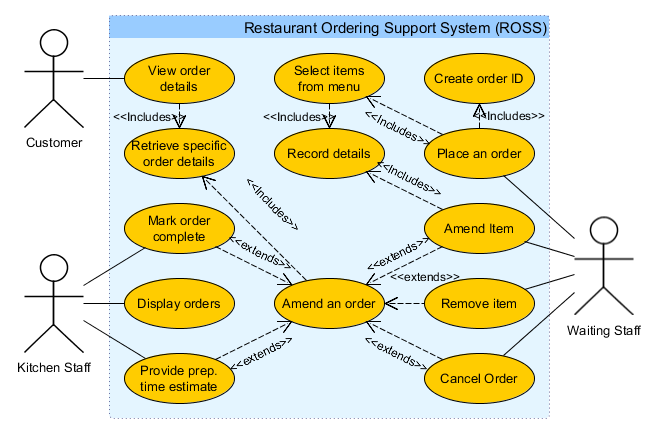
\includegraphics[scale=1]{Figures/UseCaseDiagram.png}
\caption{Use case diagram for the Restaurant Ordering Support System.}
For clarity and simplicity a one-to-one relationship with specific requirements is not enforced, and specific use cases ignore component boundaries.
\end{sidewaysfigure}


\subsection{Activity Diagrams}

\begin{figure}[H]
\centering
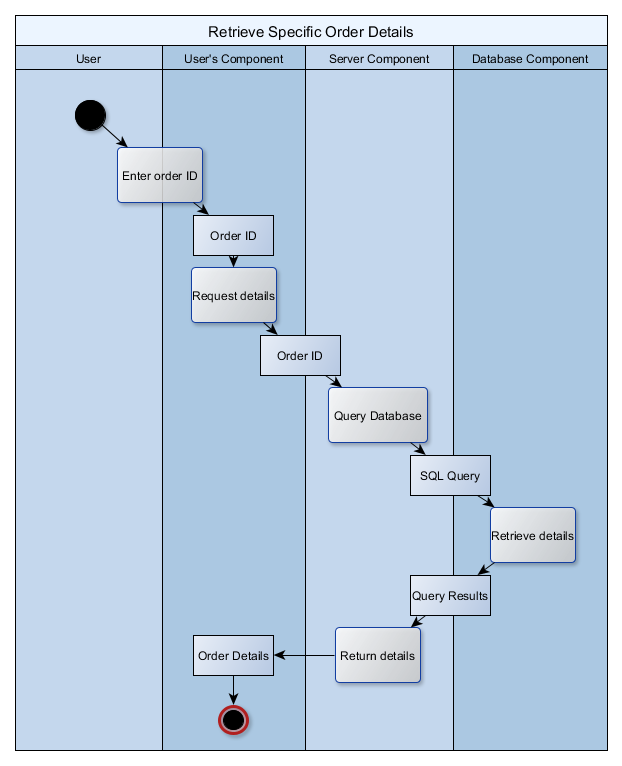
\includegraphics[scale=0.75]{Figures/RetrieveOrder.png}
\caption{A sub-activity to retrieve details of a given order.}
\end{figure}

\begin{figure}[H]
\centering
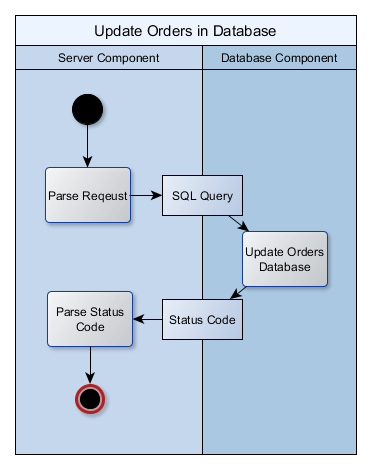
\includegraphics[scale=1]{Figures/UpdateOrderDB.png}
\caption{A sub-activity to perform an update to an order in the Database component.\newline
Updates can include adding, amending, or removing an order as well as adding prep. time estimates or marking as complete.}
\end{figure}

\begin{figure}[H]
\centering
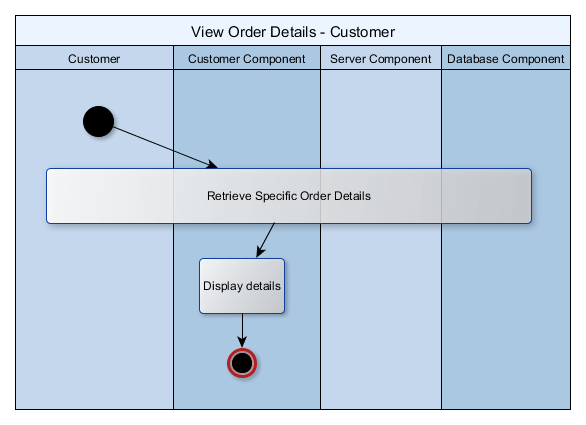
\includegraphics[scale=0.75]{Figures/CustomerViewDetails.png}
\caption{The activity diagram for a customer to view their order status.}
\end{figure}

\begin{figure}[H]
\centering
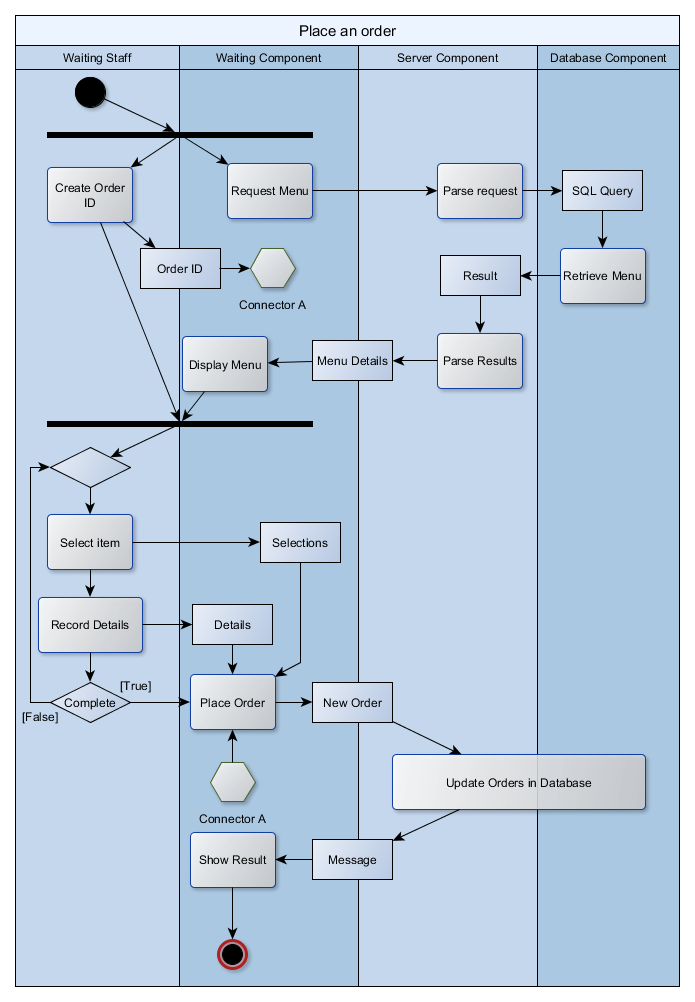
\includegraphics[scale=0.55]{Figures/PlaceOrder.png}
\caption{The activity diagram for entering an order into the system.}
\end{figure}

\begin{figure}[H]
\centering
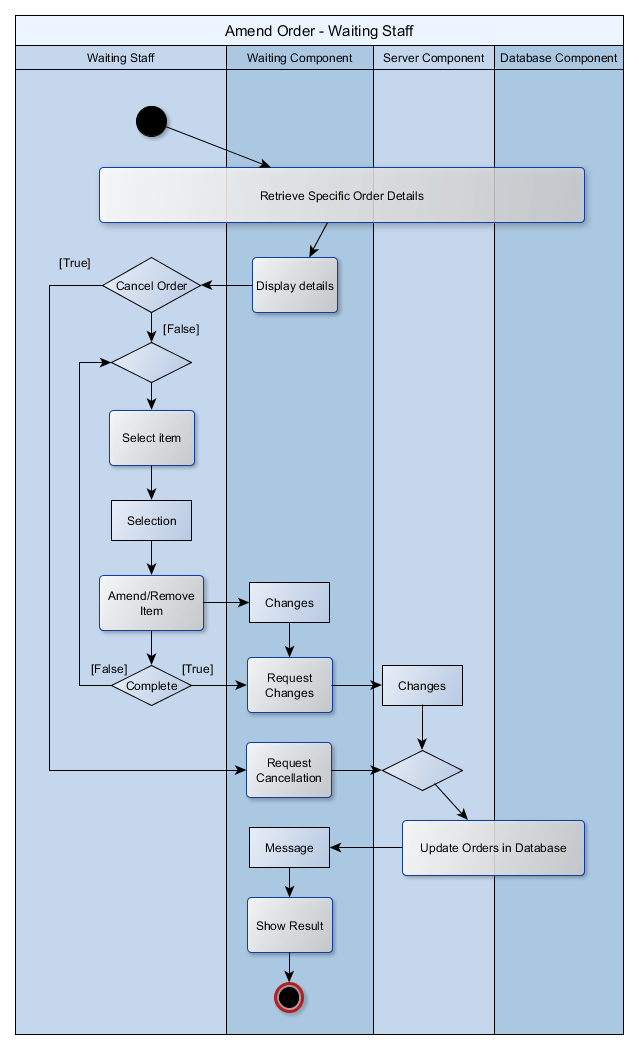
\includegraphics[scale=0.55]{Figures/WaiterAmendOrder.png}
\caption{The activity diagram representing waiting staff amending an order.}
\end{figure}

\begin{figure}[H]
\centering
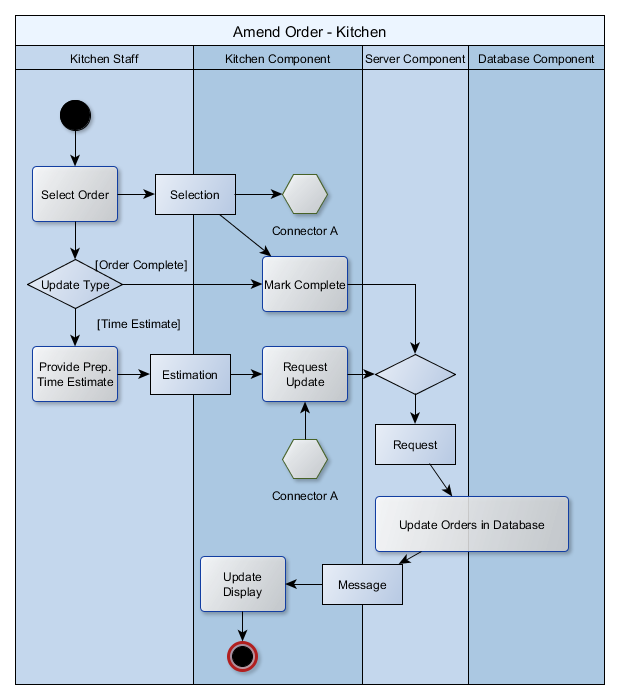
\includegraphics[scale=0.75]{Figures/KitchenAmendOrder.png}
\caption{The activity diagram representing kitchen staff amending an order.}
\end{figure}

\section{Assumptions and Dependencies} \label{subsec:Assumptions}

It is assumed that the restaurant is capable of implementing and maintaining a reliable wireless Local Area Network pursuant to any relevant requirements specified in this document.\\
It is further assumed that the restaurant has or will have an active wireless Local Area Network implemented for the installation of this system.\\
\\
It is assumed that the restaurant has or will have the ability to maintain the server hardware and software - where said software has not been implemented as part of this project - by the end of this project. This may or may not be through a Service-Level Agreement with Buzzword.\\
As a corollary, no assumptions have been made regarding the maintenance of any bespoke software written for this project - primarily the 5 components mentioned in \gref{sec:Scope}.\\
\\
It is assumed that the restaurant will take all reasonable steps to manage access to human-system interfaces, and as such little to no security measures must be implemented in this project. Human-system interfaces here refers primarily (but not exclusively) to the hardware devices to which \autoref{secure:HardwareLocking} applies. That is those hardware devices through which access-limited software components can be accessed. For example, the devices carried by waiting staff.

\section{Definition of Terms} \label{subsec:Definitions}
\vspace{1cm}

\begin{tabulary}{1.2\textwidth}{l L}
Term & Definition \\ \midrule

Server & The hardware and software environment which will provide copies of the Kitchen, Waiting, and Customer components to connected client devices. Also provides the hardware and software for execution of the Server and Database components.\newline Server does \textbf{not} refer to a waiter, waitress, or other member of staff. \\ \midrule
Client device & The device being used to interact with the system. This will be the computer used by Kitchen staff, mobile or tablet device used by waiting staff, and any customer's device which has received the Customer component of the system from the server.\\ \midrule
Local Area Network (LAN) & The collection of computer networking devices within the restaurant's premises. \\ \midrule
Prep. & Short for Preparation. In the context of the phrase "prep. time" it refers to the time taken from starting to prepare the order/item (depending on usage) to being completed.
\end{tabulary}



\nocite{*}
\printbibliography



\end{document}